\documentclass[12pt,a4paper, ngerman]{article}
\makeatletter
\def\set@curr@file#1{%
  \begingroup
    \escapechar\m@ne
    \xdef\@curr@file{\expandafter\string\csname #1\endcsname}%
  \endgroup
}
\def\quote@name#1{"\quote@@name#1\@gobble""}
\def\quote@@name#1"{#1\quote@@name}
\def\unquote@name#1{\quote@@name#1\@gobble"}
\makeatother
\usepackage[paper=a4paper,left=25mm,right=25mm,top=25mm,bottom=25mm]{geometry}
\usepackage{babel}
\usepackage{amsmath}
\usepackage[style=numeric]{biblatex}
\addbibresource{Maturarbeit.bib}
\usepackage{graphicx}
\usepackage{wrapfig}
\usepackage{listings}
\usepackage{xcolor}
\usepackage{xfrac}
\usepackage{titlesec}

\usepackage{hyperref}

\makeatletter
\newcommand{\addloflink}[1]{% \addloflink{<URL>}
  \addtocontents{lof}{\url{#1}}
}
\newcommand{\l@figlink}{\@dottedtocline{1}{1.5em}{2.3em}}
\makeatother

\definecolor{codegreen}{rgb}{0,0.6,0}
\definecolor{codegray}{rgb}{0.5,0.5,0.5}
\definecolor{codepurple}{rgb}{0.58,0,0.82}
\definecolor{backcolour}{rgb}{0.95,0.95,0.92}
 
\lstdefinestyle{mystyle}{
    backgroundcolor=\color{backcolour},   
    commentstyle=\color{codegreen},
    keywordstyle=\color{magenta},
    numberstyle=\tiny\color{codegray},
    stringstyle=\color{codepurple},
    basicstyle=\ttfamily\footnotesize,
    breakatwhitespace=false,         
    breaklines=true,                 
    captionpos=b,                    
    keepspaces=true,                 
    numbers=left,                    
    numbersep=5pt,                  
    showspaces=false,                
    showstringspaces=false,
    showtabs=false,                  
    tabsize=2
}
 
\lstset{style=mystyle}

\setcounter{secnumdepth}{4}

\titleformat{\paragraph}
{\normalfont\normalsize\bfseries}{\theparagraph}{1em}{}
\titlespacing*{\paragraph}
{0pt}{3.25ex plus 1ex minus .2ex}{1.5ex plus .2ex}

\begin{document}
\title{\large Maturitätsarbeit an der Kantonsschule Zürich Nord \\ \Huge Regelungstechnik \\ \huge PID-Parametrisierung anhand eines selbstgebauten Quadrocopters}
\author{Charpoan Kong M6d \\ Betreuer: Christian Prim}
\date{\today}
\maketitle
\pagenumbering{gobble}





\newpage
\clearpage
\pagenumbering{Roman}
\tableofcontents
\newpage
\pagenumbering{arabic}

\section{Einleitung}
Ein Quadrocopter ist ein Flugobjekt mit vier Propellern. Schon in den 1920er Jahren wurde diese Technik eingehend untersucht. Der Luftfahrtpionier Étienne \OE hmichen, der 1920 den Oehmichen No. 2 gebaut hatte, machte schon Versuch mit Flugobjekten mit vier Propellern. Damals waren die Propeller elastisch und man konnte mit Seilzügen den Anstellwinkel der Propeller einstellen. Er konnte damit einige Rekorde aufstellen.\cite{website:Wikipedia_Quadrocopter}\\ \\
In der heutigen Zeit finden Quadrocopter viele Anwendungen, wie z.B. bei Suchaktionen, im Militär oder auch als Spielzeug. Mit der schnellen Entwicklung von Mikroprozessoren wurden Quadrocopter immer kleiner und einfacher zu realisieren. Auch können damit teurere Helikopterflüge für Kartographie oder Luftaufnahmen billiger realisiert werden.\cite{website:Wikipedia_Quad_Einsatz}\\ \\
Die Intention zu dieser Arbeit folgt aus einem Projekt aus dem Freifachkurs Robotik. Damals kam der Raspberry Pi zum Einsatz. Da dieser ein Betriebsystem parallel zum Flightcontroller am laufen hat, war die Regelung des Flightcontrollers zu träge. Auch war das Stueuersignal an den Motoren viel zu zitterig und so war waren diese unbrauchbar. Desswegen wird auch ein neuer Chip evaluiert, der den Echtzeitanforderungen entspricht und eine richtige Hardware Pulsweitenmodulation (PWM) hat. \\ \\
\iffalse
Mit dieser Arbeit will ich mit dem Bau und dessen Regelung befasssen. Der Quadrocopter wird selbst gebau mit dem Hauptziel den Flightcontroller selbst zu designen, bauen und programmieren. So sollte die Regelung auch selbst implementiert werden. Dannach sollten Versuche gemacht werden, die bestimmen sollten, wie der PID-Regler stabiler gemacht werden kann und wie ungleichheiten, wie sie durch Vibration entstehen, auszugleichen. 
\fi
Die Fragestellung lautet, wie die Regelung des Flightcontrollers implementiert werden muss, damit diese funktioniert und welche Faktoren diese stören und wie schnell die Daten verarbeitet werden müssen. Auch wird untersucht , welche Lösungen es für diese Probleme gibt und es wird vcersucht diese zu implementieren. \\ \\
In der Arbeit wird der Quadrocopter selber gebaut, mit dem Hauptziel den Flightcontroller selbst zu designen und zu programmieren. Dannach werden Versuche gemacht, die bestimmten wie der PID-Regler stabiler gemacht wird und wie ungleichheiten, die durch Vibrationen enstehen, ausgeglichen werden können. Die Fernbedienung wird auch selbst gebaut und dient auch dazu Daten wärend des Fluges auszuwerten. 
\newpage
\section{Theorie}
\subsection{Funktionsweise eines Quadrocopters}
Man könnte meinen, dass man einen stabilen Flug erreichen kann, wenn der Schub der vier Rotoren gleich ist. Aber dies ist leider nicht möglich, da viele Umwelteinflüsse einen stabilen Zustand verhindern wie z.B. Wind, unterschiede in den Rotoren oder Motoren, Assymetrie des Rahmens etc. So muss ein Computer, der Flightcontroller (FC), das Gleichgewicht erhalten, indem dieser den Schub der vier Motoren so regelt, dass der Quadrocopter im Gleichgewicht ist oder dieser einen anderen bestimmten Winkel hält.\\
\begin{figure}[h]
\centering
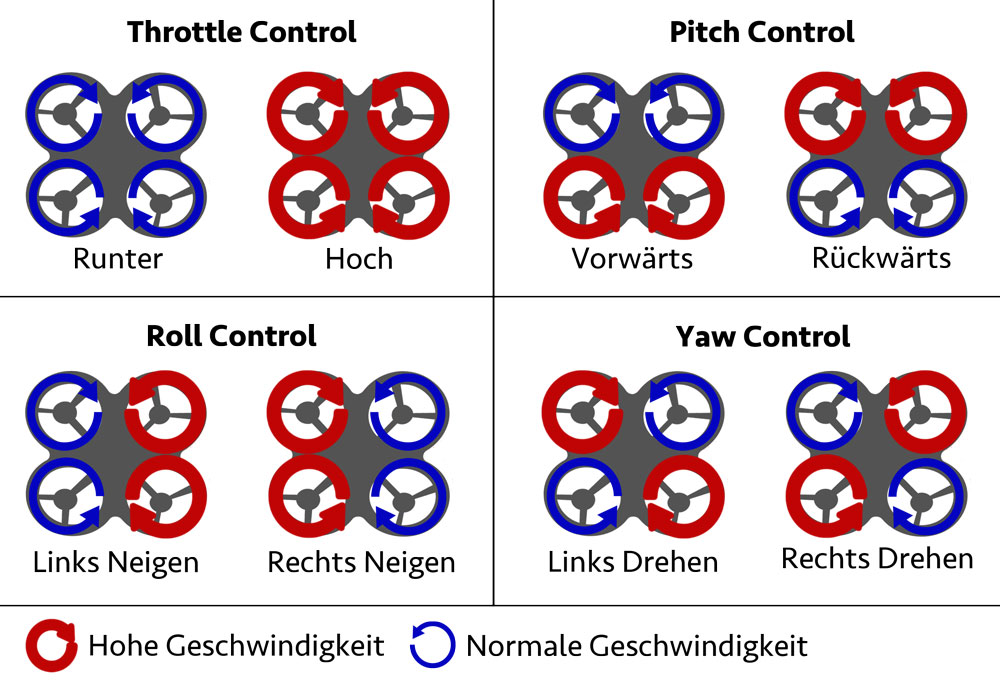
\includegraphics[width=\textwidth]{MotionDE.jpg}
\caption[\url{http://fpvracing.ch/img/cms/MotionDE.jpg}]{Drehrichtung und Schub bei verschiedenen Steuereingaben }
\end{figure}\\
Abbildung 1 zeigt die Rotationsrichtung der Motoren. Die benachbarten Motoren müssen eine gegensätzliche Rotation haben, da sonst der Quadrocopter ins Rotieren gerät. So wird das Drehmoment des anderen Motors ausgeglichen. Auch wird gezeigt, dass man den Quadrocopter mit erhöhen bzw. erniedrigen der Motorleistung der richtigen Motoren, diesen in die gewünschte Richtung steuern kann. Kernelement dieser Steuerung ist der PID-Regler.
\newpage
\subsection{Was ist ein Regler?}
Eine Regelung ist eine Steuerung mit Rückkoppelung. Ein Wert z.B. die Drehzahl eines Motors überwacht und je nach gewünschter Drehzahl, das Drehmoment des Motors geregelt, dass er auch diesen halten kann, auch wenn eine Last am Motor hängt.\cite{website:rn-wissen_Regelungstechnik}\\
\begin{wrapfigure}[6]{r}{0.4\textwidth}
\centering
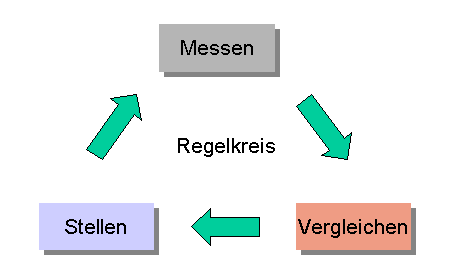
\includegraphics[width=0.4\textwidth]{Regelkreis1.png}
\caption[\url{https://rn-wissen.de/wiki/images/2/25/Regelkreis1.png}]{Der Regelkreis}
\end{wrapfigure}
Im Reglekreis (siehe Abb.2) wird der Ist-Wert z.B. mit einem Sensor gemessen. Dieser wird mit dem Soll-Wert verglichen, um die Regelabweichung zu bestimmen. So kann die Reglegrösse bestimmt werden, um so das System dem Soll-Wert anzugleichen.\\ \\ \\ \\ \\ \\ \\
Die Regelabweichung kann dabei einfach mit der Differenz des Ist-Wertes $x$ mit dem Soll-Wertes $w$ bestimmt werden.\cite{website:rn-wissen_Regelungstechnik}
\begin{equation}
e(t)=w-x
\end{equation}\\

\begin{wrapfigure}[8]{l}{0.4\textwidth}
\centering
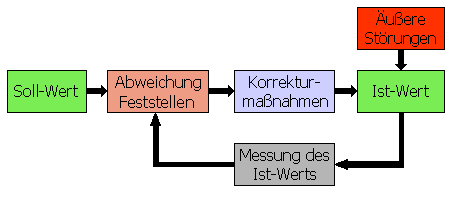
\includegraphics[width=0.4\textwidth]{Regelkreis2.png}
\caption[\url{https://rn-wissen.de/wiki/images/5/5d/Regelkreis2.png}]{Wirkungsweise des Regelkreises}
\end{wrapfigure}
\noindent
In Abbildung 3 sieht man, wie vorher beschrieben, wie ein solcher Regelkreis funktionert. In der Regelungstechnik wird versucht einen solchen Regelkreis mathematisch zu modellieren. In diesem Kapitel wird nur der PID-Regler und seine Komponenten besprochen, da dieser häufig bei Quadrocoptern benutzt wird.\cite{website:rn-wissen_Regelungstechnik}
\\ \\ \\ \\
Der PID-Regler besteht aus mehreren Relgern und dem D-Glied. In der Folge wird beschrieben wie die einzelnen Komponenten wirken. 

\subsubsection{P-Regler}
Der P-Regler wirkt linear. Dieser Regler gibt die Regelabweichung verstärkt und unverzögert mit dem Faktor $Kp$ weiter (Vgl. \ref{p}). Das Problem dabei ist, dass diese Abweichung bleibend ist und somit den Soll-Wert über- bzw. unterschiesst. Dieser Regler wirkt schnell.\cite{website:rn-wissen_Regelungstechnik}
\begin{equation}\label{p}
y(t)=Kp\cdot e(t)
\end{equation}
\newpage
\subsubsection{I-Regler}
Beim Integralregler wird die Regelabweichung über die Zeit summiert und mit dem Faktor $Ki$ verstärkt (Vgl. \ref{i}). Dabei werden Abweichungen volständig eliminiert, da dieser Regelwert immer anwächst, solange die Regelabweichung nicht Null ist. Dieser Regler wirkt langsam.\cite{website:rn-wissen_Regelungstechnik}\\
\begin{equation}\label{i}
y(t)=Ki\int_{0}^{t}e(t)dt
\end{equation}

\subsubsection{D-Glied}
Das Differenzialglied schaut auf die Differenz der Regelabweichung zur vorherigen Regelabweichung und wird mit dem Faktor $Kd$ verstärkt (Vgl. \ref{d}). Desshalb reagiert dieser sehr schnell und gibt den beiden anderen Vorhaltezeit.Differenzialglied ist kein Regler da es alleine nichts regleln kann, sondern nur auf Veränderungen in der Regelabweichung reagiert.\cite{website:rn-wissen_Regelungstechnik}\\
\begin{equation}\label{d}
y(t)=Kd\cdot \dot{e}(t)
\end{equation}

\subsubsection{PID-Regler}
Beim PID-Regler werden die Eigenschaften der einzelnen Regler und dem D-Glied vereint (Vgl. \ref{pid}).
\begin{equation}\label{pid}
y(t)=Kp\cdot e(t)+Ki\int_{0}^{t}e(t)dt+Kd\cdot \dot{e}(t)
\end{equation}
\newpage
\subsection{Digitaler Low-Pass Filter}
Ein Low-Pass Filter filtert hohe Frequenzen heraus. Der Filter ist aus der Elektronik oder der Tontechnik bekannt. Beim Quadrocopter wird ein solcher Filter für das Unterdrücken des Rauschens des Inertialsensors verwendet. Dieses Rauschen wird durch die Vibrationen der Motoren erzeugt und liegt ca. bei 133Hz.\\ \\
Beim vorliegenden Digitalen Low-Pass Filter (DLPF) wird ein analoger RC-Low-Pass Filter emuliert, wie der in Abbildung 4.\cite{website:Wikipedia_LPF}\\ \\
Im letzten Kapitel wurde der PID-Regler eingeführt, doch Vibrationen verursachen Störungen in der Regelung und führen so zu falschen Korrekturen. Zum Beispiel verursachen diese beim D-Glied starke Auschläge, wenn diese hohe Amplituden haben. Auch wird dieser dann unbrauchbar, da die Regelabweichung durch die Vibrationen verfälscht wird. Ein Filter versucht diese Vibrationen zu dämpfen und verhindert so, starke Ausschläge.
\begin{figure}[h]
\centering
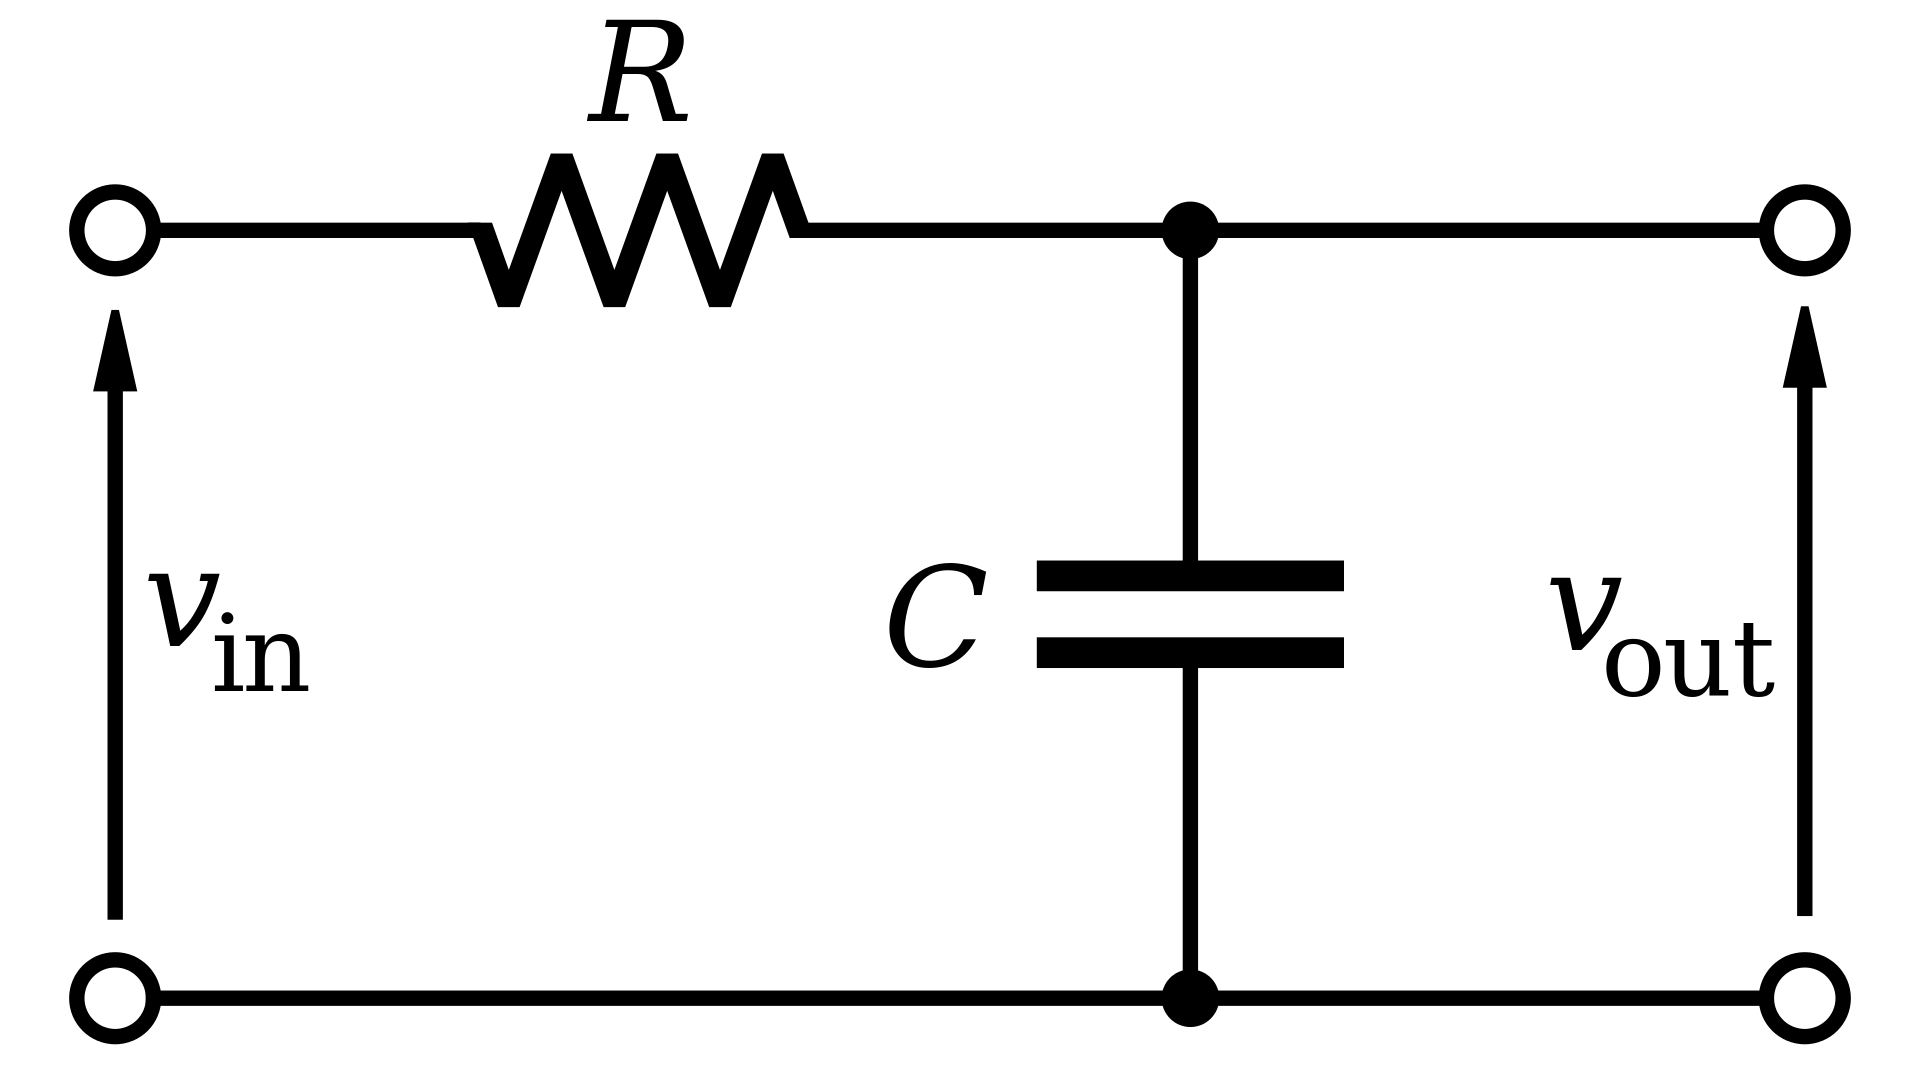
\includegraphics[width=0.4\textwidth]{DLPF1.png}
\caption[\url{https://upload.wikimedia.org/wikipedia/commons/e/e0/1st_Order_Lowpass_Filter_RC.svg}]{RC Low-Pass Filter}
\end{figure}\\
Wie man in \ref{eq1} sieht, ist die Eingang- und Ausgangsspannung vom Widerstand und von der Stromstärke abhängig.
\begin{equation} \label{eq1}
v_{\text{in}}(t)-v_{\text{out}}(t)=R\cdot I(t)
\end{equation}
Der Strom kann man auch abhängig vom Kondensator und der Ausgangsspannung darstellen, wie man in \ref{eq2} und \ref{eq3} sieht.
\begin{equation} \label{eq2}
Q_{c}(t)=C\cdot v_{\text{out}}(t)
\end{equation}
\begin{equation} \label{eq3}
I(t)=\dot{Q}_{c}(t)=C\cdot \dot{v}_{\text{out}}(t)
\end{equation}
So kann man die Differenzialgleichung \ref{eq1} wie \ref{eq111} darstellen.\\
\begin{equation} \label{eq111}
v_{\text{in}}(t)-v_{\text{out}}(t)=RC\cdot \dot{v}_{\text{out}}(t)
\end{equation}
Jetzt wird $v_{\text{in}}(t)$ mit $x_{i}$ und $v_{\text{out}}$ mit $y_{i}$ dargestellt und die Differenzialgleichung diskretisiert zu der Differenzengleichung \ref{eq4}.
\begin{equation}\label{eq4}
x_{i}-y_{i}=RC\cdot \frac{y_{i}-y_{i-1}}{\Delta t}
\end{equation}
\newpage
\noindent
Die Gleichung \ref{eq6} (Ganze Auflösung siehe Anhang 1 Auflösung 1) wird nach $y_{i}$ umgeformt und man kann $\sfrac{\Delta t}{\Delta t+RC}$  mit $\alpha$ und $\sfrac{RC}{\Delta t + RC}$ mit $\alpha-1$ substituieren wie in \ref{eq5} gezeigt.
\begin{equation} \label{eq6}
y{i}=x_{i}\frac{\Delta t}{\Delta t+RC} + y_{i-1}\frac{RC}{\Delta t+RC}
\end{equation} 
\begin{equation}\label{eq5}
y{i}=\alpha x_{i} + (1-\alpha)y_{i-1} \quad \text{mit} \quad \alpha:=\frac{\Delta t}{\Delta t+RC}
\end{equation}
$RC$ kann mit der Formel für den Low-Pass Filter durch $f_{c}$ dargestellt werden wie unten gezeigt wird.
\begin{align*}
f_{c} = \frac{1}{2\pi RC} \\
RC = \frac{1}{2\pi f_{c}} 
\end{align*}
Jetzt kann auch das $RC$ in der Definition von $\alpha$ ersetzt werden, damit die Gleichung nicht mehr von $RC$ abhängig ist (Ganzer Beweis siehe Anhang 1 Beweis 1).
\begin{equation*}
\alpha = \frac{2\pi f_{c}\Delta t}{1+2\pi f_{c}\Delta t} 
\end{equation*}
\newpage
\section{Versuchsaufbau}
\subsection{Quadrocopter}
\subsubsection{Motoren}
Die verwendeten Motoren sind sogenannte bürstenlose Motoren. Diese werden mit einem Electronic Speed Controller (ESC) angesteuert, dieser wandelt die Steuerimpulse in die richtige Spannung für den Motor. Da ihre RPM von Spannung abhängig ist, wird einen $Kv$-Wert angegeben. So kann man mit der Formel
\begin{equation}
a=Kv\cdot U \quad mit \quad [a]=\text{rpm}
\end{equation}
die Rotationen pro Minute berechnen.\\ \\
Beim vorliegenden Quadrocopter handelt es sich um ReadyToSky RS2205 Motoren mit einem $Kv$ von 2300. Diese Motoren wurden ausgesucht, da sie für genug Leistung bringen für einen Quadrocopter mit einer Rahmenlänge von 250mm.
\subsubsection{Akku}
\begin{wrapfigure}[10]{r}{0.4\textwidth}
\centering
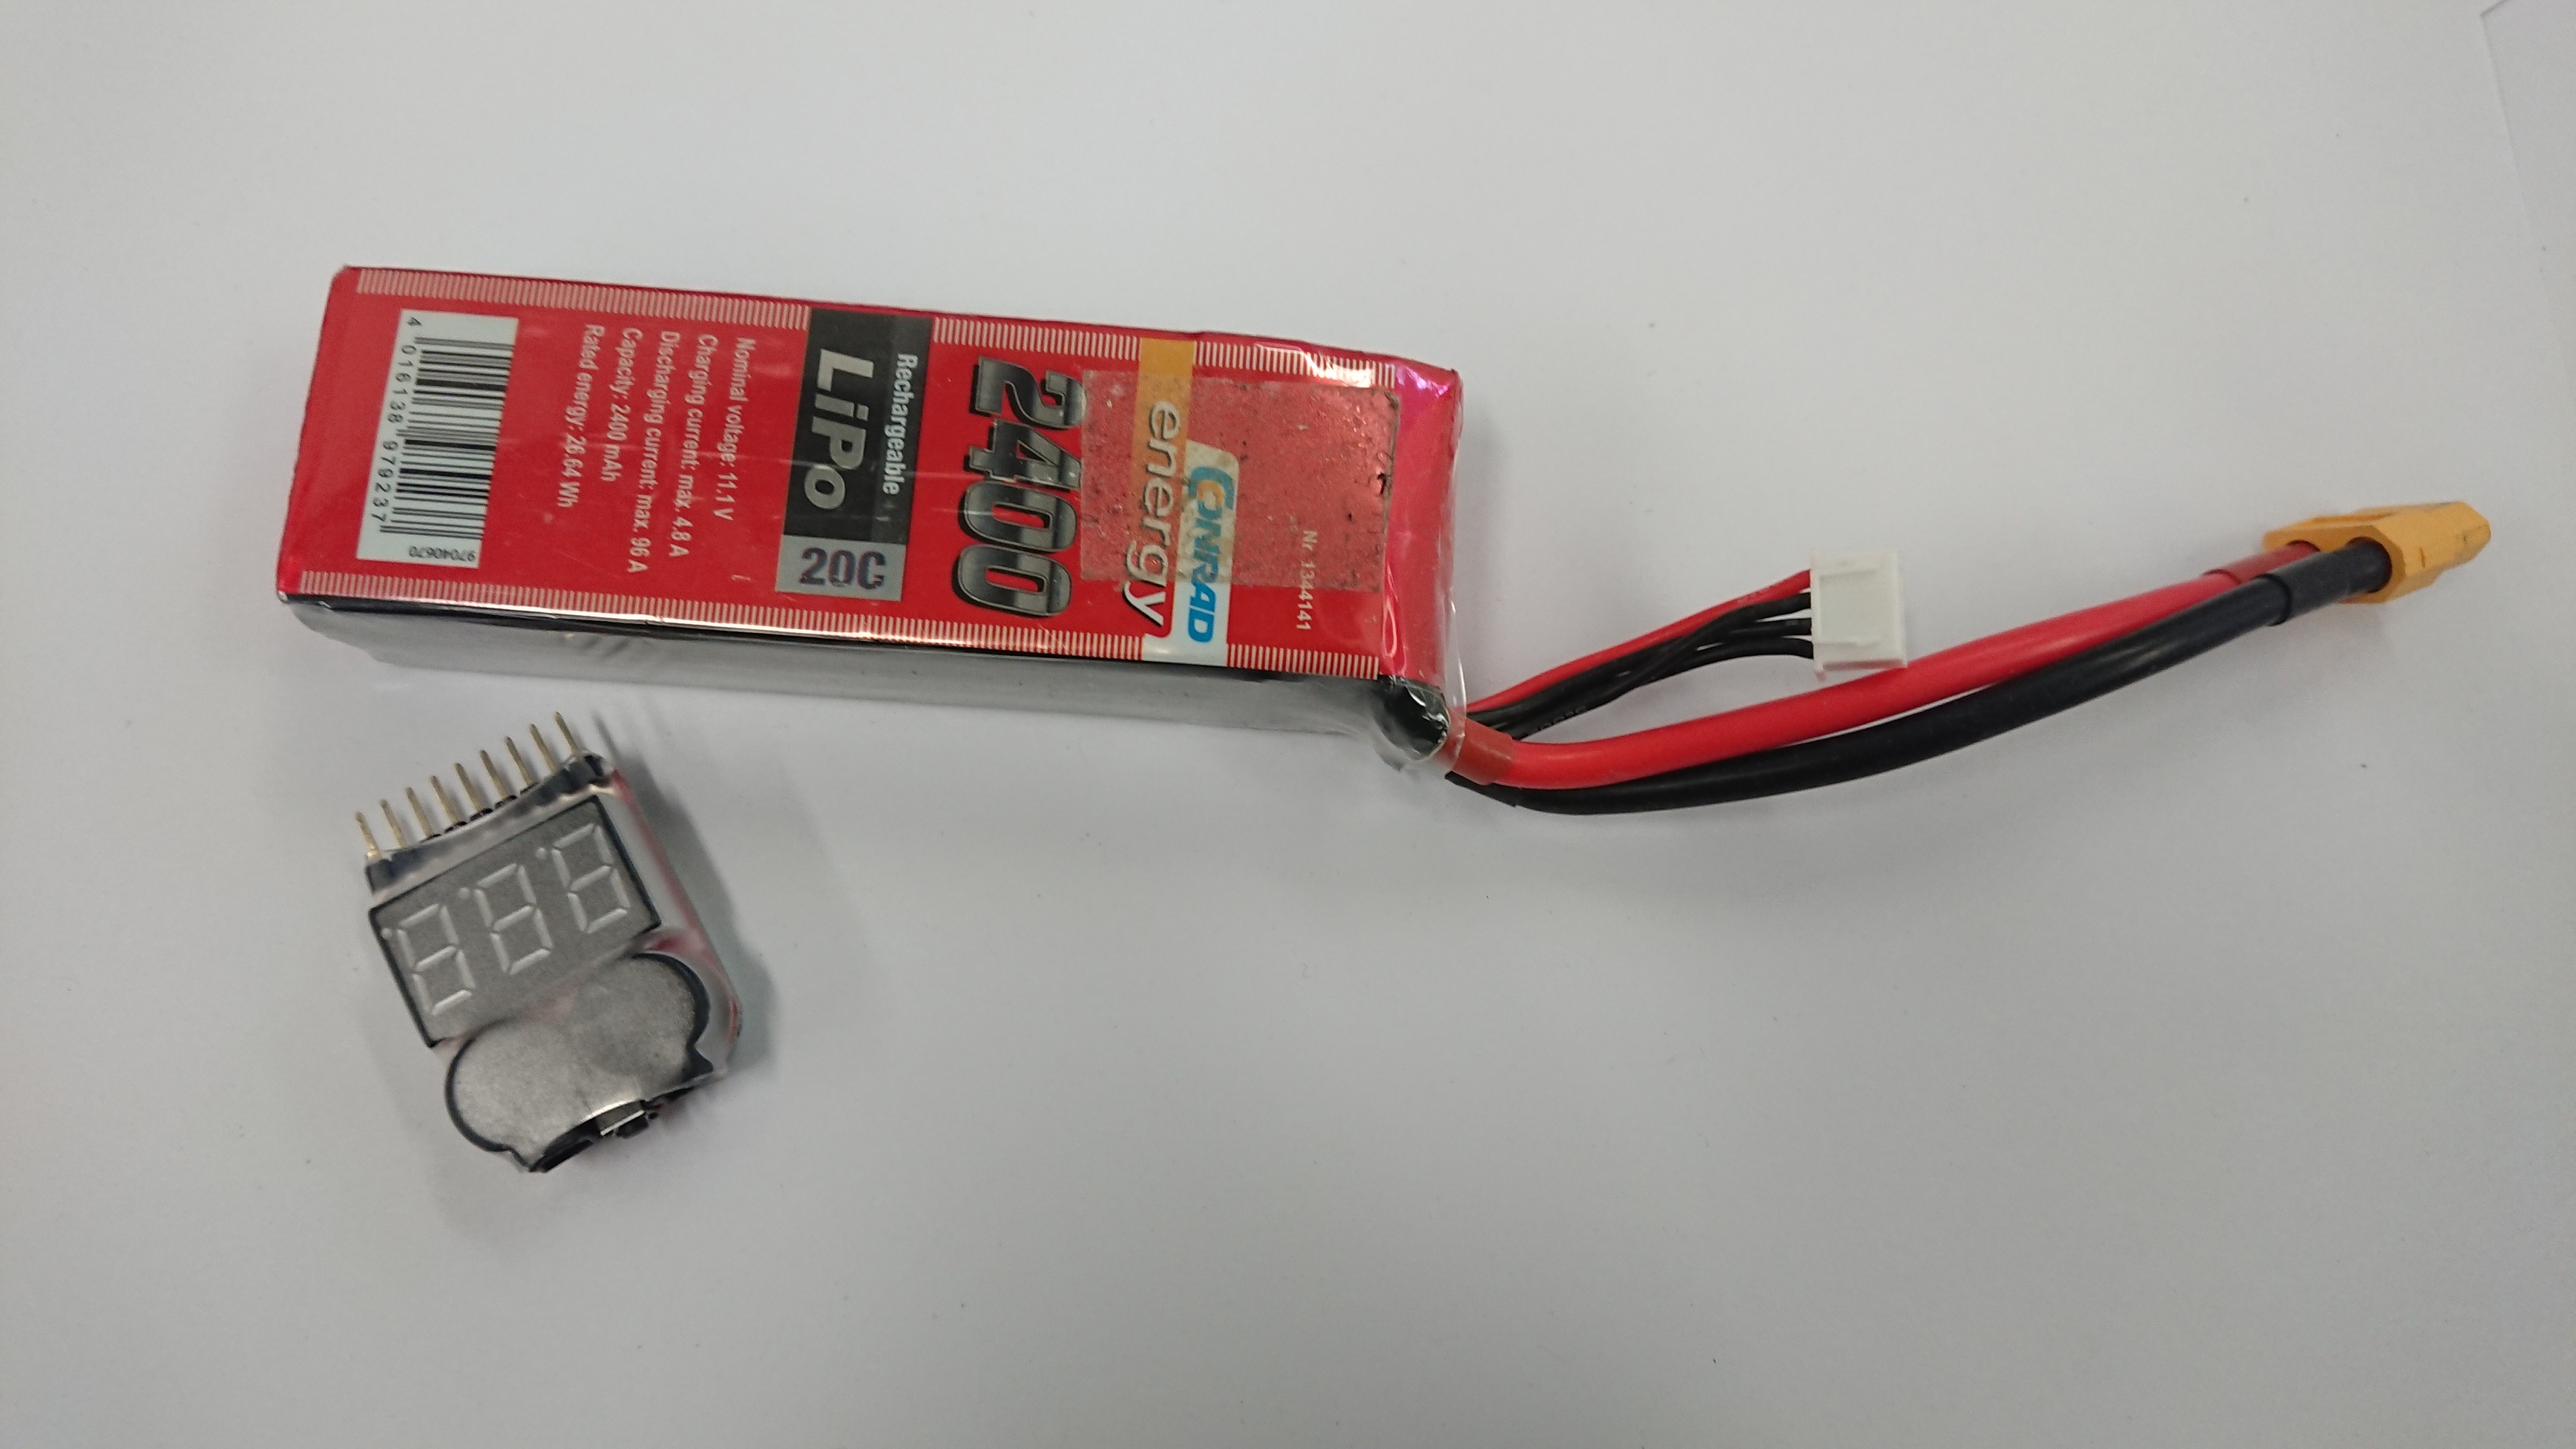
\includegraphics[width=0.4\textwidth]{accu.jpg}
\caption[Eigenes Bild]{LiPo-Akku und Akkuüberwacher} \label{accu}
\end{wrapfigure}
Der Akku (Abb.\ref{accu}) versorgt alle Komponenten, die Strom brauchen mit Strom. Im Quadrocopter wird ein LiPo Akku benutzt, der drei Zellen in Serie geschaltet hat mit einer Kapazität von 2.4Ah. Die miminale Spannung beträgt 11.1V. Die Entladerate wird $C$-Rate angegeben. Mit der Kapazität multipliziert wird der maximale Entladestrom ausgerechnet.\cite{website:fpvracing.ch_Mult_Komp}
\begin{equation}
I_{\text{max}}=Q\cdot C
\end{equation}\\ \\
Man benutzt in Quadrocoptern meist LiPo Akkus, da sie eine hohe Energiedichte besitzen und viel Leistung abgeben können. Dies aber hat auch zur Folge, dass man diese Akkus sorgfältig behandeln muss, da sie im Extremfall, Feuer fangen oder explodieren können. So darf man die einzelnen Zellen nicht unter einer Spannung von 2.7V fallen lassen. Desshalb wird der Akku auch an einem Akkuüberwacher angeschlossen, der piepst, wenn der Akku verbraucht ist. Auch braucht man ein Balanceladegerät, das kontrolliert, dass alle Zellen gleichmässug geladen werden. Eine hohe Kapazität garantiert nicht immer eine längere Flugzeit, da mehr Kapazität auch mehr Gewicht bedeutet.\cite{website:fpvracing.ch_Mult_Komp}
\newpage

\subsection{Der Flightcontroller}
Der Flightcontroller ist das Herz des Quadrocopter. Dieser liest alle Sensoren und gibt den ESCs die Steuerimpulse. In dem Kapitel wird zuerst in die wichtigsten Komponenten eingegangen, dann wird der Design-, Bau und Propgrammierprozess beschrieben.
\subsubsection{Komponenten}
\paragraph{Microcontroller}
Der Microcontroller, der auf dem FC benutzt wird, ist ein ARM-Cortex-M7 STM32F722RET6 Microcontroller von STMicroelectronics. Dieser besitzt alle Schnittstellen um die einzelnen Sensoren und andere Komponenten auszulesen und anzusteuern. Da dieser nicht genug Pins hat, wird noch ein zweiter Microcontroller benutzt und zwar der ATMega328P, der auch auf dem Arduino/Genuino UNO zu finden ist. Dieser liest den Drucksensor und einige ADCs aus und kommuniziert mit dem I2C-Protokoll mit dem STM32. \\ \\
Microcontroller können anders als Mikroprozessoren, der auf dem Raspbery Pi verbaut ist, ohne Zusatz Pehpetrie benutzt werden, da sie schon einen Flash, RAM oder ähnliches besitzen. 

\paragraph{Sensoren}
Die wichtigsten Sensoren des Quadrocopter sind der Gyrosensor und der Beschleunigungssensor. Der Gyrosensor misst die Winkelbeschleunigung der Achsen. In dem FC wurde eine ICM-20689 von TDK InvSense benutzt. Dieser hat beide Sensoren in einem Chip integriert und wird per SPI-Protokoll ausgelesen. Als Backup wird ein MPU-6050 benutzt, auch vom gleichen Hersteller, dieser wird mit dem langsameren I2C-Protokoll ausgelesen. \\
\begin{wrapfigure}[10]{r}{0.5\textwidth}
\centering
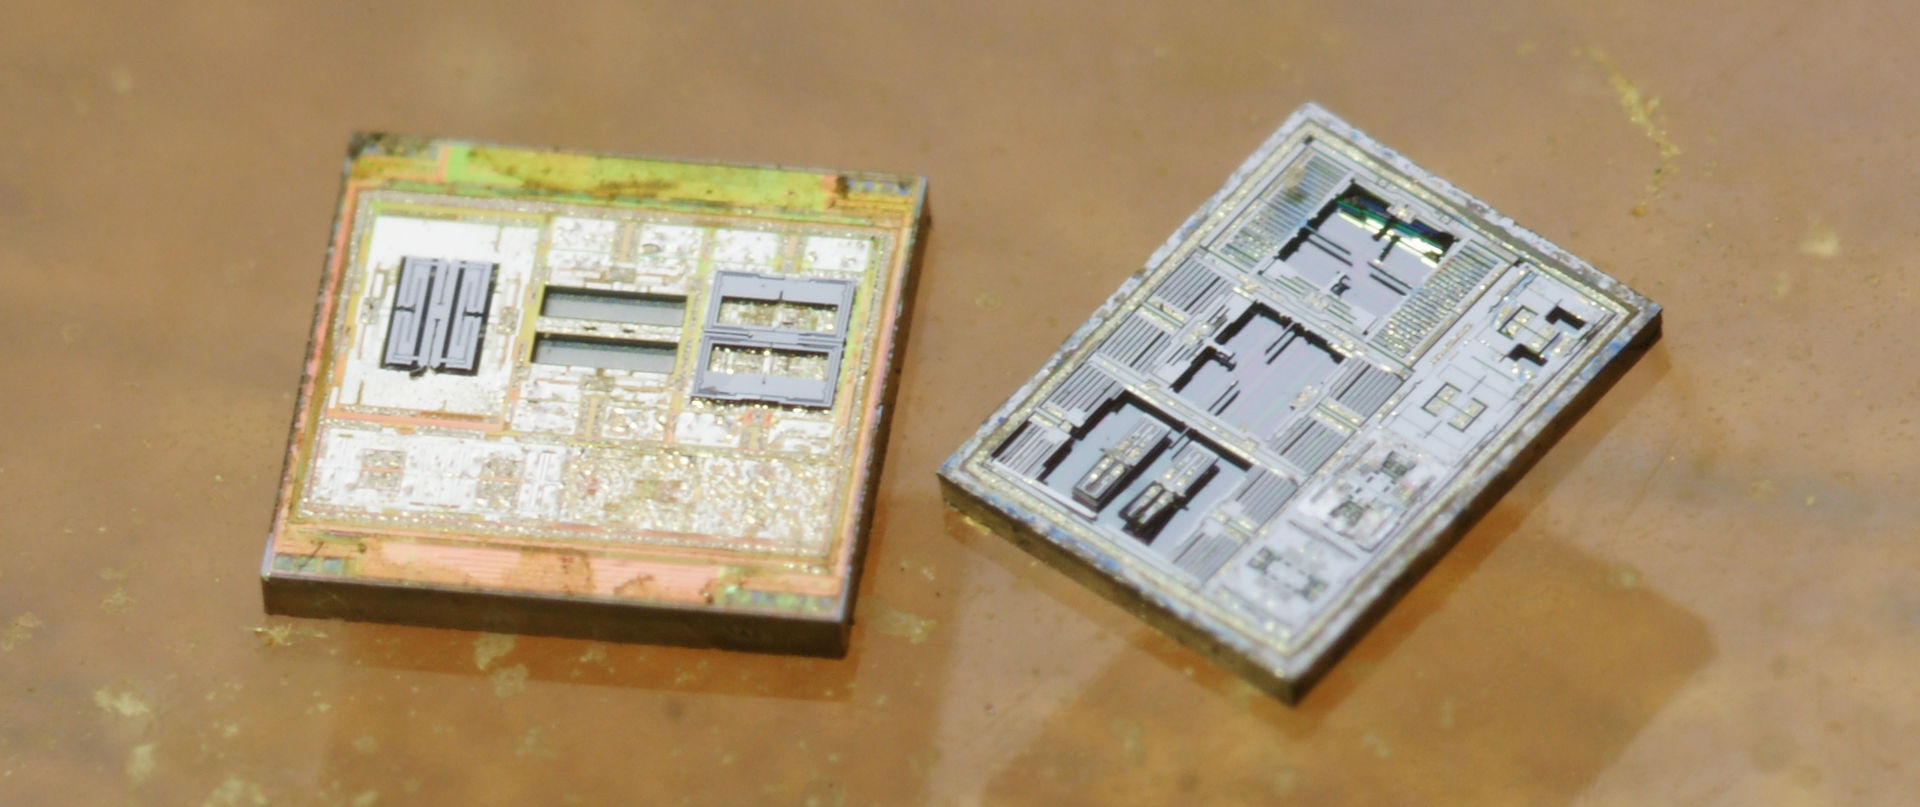
\includegraphics[width=0.5\textwidth]{1920px-Mpu6050-HD.jpg}
\caption[\url{https://upload.wikimedia.org/wikipedia/commons/2/27/Mpu6050-HD.jpg}]{Dice des MPU6050}
\end{wrapfigure}
Beide sind sogenannte MEMS-Sensoren. MEMS bedeutet microelectromechanical systems. Das bedeutet, dass diese Sensoren auf einer mechanischen Basis funktionieren.\cite{website:elek_Komp_MEMS}. Man ätzt die Sensorstrukturen und deren auslese Schaltung auf einen Chip. Abbildng 5 zeigt die eingeätzte Siliziumstruktur des MPU6050.\\ \\
Da der Gyrosensor nur Winkelgeschwindigkeit, bei den Sensoren $\frac{^\circ}{s}$ und nicht $\frac{rad}{s}$ misst, muss diese noch mit der Loop-Zeit multipliziert werden, um den Winkel zu bekommen (vgl. \ref{aaa}).
\begin{equation}\label{aaa}
w=\omega\cdot dt \quad mit \quad [w]=^\circ \quad und \quad [\omega]=\frac{^\circ}{s}
\end{equation}
Wenn man den Absoluten Winkel alleine mit dem Gyrosensor misst hat dieser über die Zeit einen Drift. Der durch das Rauschen des Sensors verursacht wird. Auch kann nicht der Anfangswinkel bestimmt werden, da dieser nur die Winkelgeschwindigkeit misst und somit keine Referenz zum Normalvektor hat, somit müsste der Quadrocopter immer von einer horizontalen Ebene starten. Deswegen braucht man da den Beschleunigungssensor. Dieser misst die Beschleunigung auf allen Achsen relativ zur Erdbeschleunigug. Beim Stillstand auf einer horizontalen Ebene misst er also
$
\begin{pmatrix}
0\\ 
0\\ 
1
\end{pmatrix}
\vec{g}
$. Man kann einfach die Norm des Beschleunigungsvektors $\vec{a} = \begin{pmatrix}
a_{x}\\ 
a_{y}\\ 
a_{z}
\end{pmatrix}$ nehmen und mit der Beschleunigung an der gewünschten Achse verrechnen, um dann den Winkel zu bekommen (vgl. \ref{gangle}).
\begin{equation}\label{gangle}
w=\arcsin(\frac{a_{x,y}}{\vec{a}}
)
\vec{g}\cdot \frac{180}{\pi} \quad mit \quad [w]=^\circ
\end{equation}
Nebenbei muss man beachten, dass C/C++ den Winkel in $rad$ berechnet und man diesen noch zu $grad$ konvertieren muss. So hat man den absoluten Winkel mit zwei Sensoren gemessen und muss diese nur noch Kombinieren. Dies geschieht mit Hilfe des Komplementärflilters(vgl. \ref{comp}). (Man muss auch beachten, dass der Absolute Winkel nur für die Nick-und Rollachse berechnen kann da, für die Gierachse noch ein Magnetometer für eine Null-Referenz nötig wäre (Achsenbezeichnung siehe Abb.\ref{ypr}).
\begin{equation}\label{comp}
w_{\text{komp}}=0.9996\cdot w_{\text{Gyro}}+0.0004\cdot w_{\text{Accl}} \quad mit \quad [w]=^\circ
\end{equation}
\begin{figure}[h!]
\centering
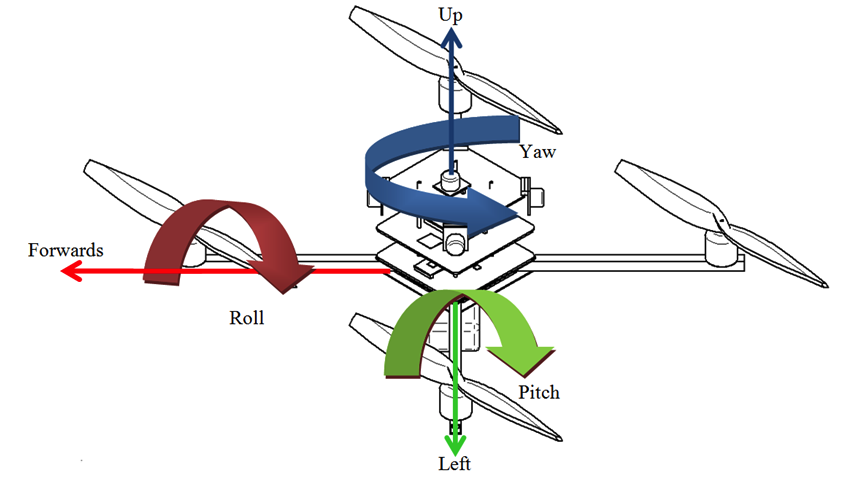
\includegraphics[width=0.5\textwidth]{ypr.png}
\caption[\url{https://technikblog.ch/wp-content/uploads/2013/03/Roll-Pitch-_Yaq-Quadcopter.png}]{Achsen des Quadrocopters. Pitch ist Nickachse und Yaw die Gierachse.}\label{ypr}
\end{figure} \\
Theoretische Überlegungen führen dazu, dass dem Winkel aus dem Beschleunigungssensor ein tiefer Faktor gegeben, da dieser Winkel nicht mehr genau stimmen wird, wenn der Quadrokopter in eine Richtung beschleunigen würde, dies wird erst bei starken Beschleunigungen der Fall sein, sonst stimmt dieser Wert ungefähr. Aber so kann man den Anfangswinkel des Quadrokopter bestimmen, ihn auch aus der Hand starten lassen und bekommt auch noch stabilere Werte.\\ \\
Desweiteren muss auch noch beachtet werden, dass bei einer Bewegung um die Gierachse, der Sensor keine Bewegung auf der Roll- und Nickachse misst. Desshalb müssen die Werte dieser Achsen bei einer Bewegung um die Gierachse mithilfe der Rotationsmatrix (vgl. ref{rotmax}) ineinander übersetzt werden.
\begin{equation}\label{rotmax}
\binom{pitch'}{roll'}=\begin{pmatrix}
\cos(\alpha) & -\sin(\alpha)\\ 
\sin(\alpha) & \cos(\alpha)
\end{pmatrix}*\binom{pitch}{roll}
\end{equation}
Somit muss man die Achsen wie folgt verrechnen (vgl \ref{pp} und \ref{rr}).
\begin{align}
roll' = \sin(\alpha)*pitch \label{pp}\\
pitch'= \sin(\alpha)*roll \label{rr}
\end{align} 

\paragraph{Empfänger}
Als Empfänger wir ein NRF24L01 Breakoutboard mit PA und LNA benutzt. Das ist ein 2.4GHz Sender und Empfänger der Firma Nordic Semiconductor. Die Kommunikation erfolgt digital und der Chip besitzt auch eine Zyklische Redundanzprüfung (CRC). Damit wird kontrolliert, ob ein Datenpaktet fehlerhafte Bits besitzt. Allenfalls wird es repariert oder verworfen. PA heisst Power Amplifying und bedeutet, dass das Signal verstärkt wird und so grössere Reichweiten erreicht werden können und LNA bedeutet Low Noise Amplifying und bedeutet, dass schwache Empfangssignale verstärkt werden.\cite{website:electronics.stackexchange.com_WhatisPALNA} Vom Hersteller wird eine Reichweite von bis zu einem Kilometer versprochen aber in einer Wohnsiedlung kommt man mit Sichtkontakt bis zu 300m, was ausreichend ist.

\subsubsection{Leiterplatte}
Auf Leiterplatte oder auch Printed Circuit Board (PCB) wird die Schaltung des FC realisiert. Dieses besteht aus Kunststoff mit den aufgeätzten Kupferbahnen und den verzinnten Lötstellen.
\paragraph{Design}
\iffalse
Zuerst habe ich mir überlegt was für einen Microcontroller ich wählen sollte. Bei meinen ersten Versuchen mit dem Raspberry gingen schief, da der Regler nicht schnell genug reagierte und eine nicht konstates Regelverhalten gezeigt hat. Einerseits lief ein Betriebsystem pararell zum Flightcontroller, adererseits war die Regelung nicht Echtzeit genug. Desswegen habe ich im Internet nachgeschaut was für Microcontroller auf den meisten Quadroopter verbaut sind. Dort werden  meist MCU aus der STM32-Familie verwendet. So kam ich auf die Webseite von Oscar Liang\footnote{\label{foot:1}https://oscarliang.com/f1-f3-f4-flight-controller/ aufgerufen am 31.03.2019} bei der die einzelnen MCU-Generationen aufgelistet waren mit den Vor-und Nachteilen. Ich entschied mich für die neuste Generation aus dieser MCU-Familie, einen STM32F7xx MCU zu benutzen. Nachher habe ich vorhandene Boards angschaut und gesehen, das die meisten den STM32F722RET6 benutzen aus dieser MCU-Generation. Als nächstes überlegte ich mir was für einen Gyro-und Beschleunigungssensor ich bentzen wolle. Ich habe schon eine MPU-6050 IMU aber ich wollte noch einen mit SPI-Protokoll, da dies schneller ist, und der andere als Backup, so recherchierte ich was für IMU's die FC's benutzen\footnote{\label{foot:2}https://blog.dronetrest.com/inertial-sensor-comparison-mpu6000-vs-mpu6050-vs-mpu6500-vs-icm20602/ aufgerufen am 31.03.2019} und entschied mich für den ICM-20689. Als Empfänger habe ich einen nRF24L01 PA + LNA gewählt.Als Backup wird noch ein PPM Eingang eingebaut für die standart Funkübertragung über eine normale Fernbedienung. Da für die Versuche Daten gebraucht werden, wird eine microSD-Karten Schnittstelle eingebaut, um die Daten aufzuzeichnen. Damit der Flightcontroller mit dem PC kommunizieren kann um zu Debuggen muss ein FTDI-Chip (F232RL) eingebaut werden damit wird das UART-Protokoll, in ein für den PC verständliches Protokoll übersetzt. Um die Höhe zu bestimmen habe ich mich für den BMP280 Drucksensor ausgewählt um die barometrische Höhe zu bestimmen. Da dieser für das auslesen eine lange Zeit braucht habe ich überlegt noch eine NebenMCU einzubauen. Deshalb habe ich den ATMega328 gewählt da er auch auf den Arduino UNO drauf ist und ich mich damit schon auskenne. Über diese MCU werden auch die Ultraschallsensoren ausgelesen, die eine genauere Höhenmessung ermöglicht, aber nur bis zu sechs Metern. Da die ESC's einen 5V Versorgungsausgang haben muss noch ein Spannungsregler  eigebaut werden, da die meisten IC's 3.3V braucchen, der Schulmechaniker Herr Thurnherr hat mir den LM3940 empfohlen.
\fi
Zuerst wurde überlegt, was für ein Microcontroller benutzt werden sollte. Bei den ersten Versuchen wurde ein Raspberry Pi benutzt, dort gingen die Versuche schief, da dieser kein konstantes Regelverhalten aufzeigte und dessweiteren ein Betriebsystem neben dem Flightcontroller lief. Ausserdem war das PWM Signal für die ESC's nicht gut und zitterten. Desswegen wurde im Internet erkundigt, was für Microcontroller in den meisten Quadrocopter verbaut sind. So wurde die Webseite von Oscar Liang entdeckt \cite{website:OS_MCU_COLL}. Dort waren die einzelnen Microcontroller mit ihren Vor-und Nachteilen aufgelistet. Für die Arbeit wurde entschieden einen STM32F7xx Microcontroller zu benutzen. Als nächstes wurde überlegt, was für ein Gyro-und Beschleunigungssensor benutzt werden sollte. Vom letzten Versuch blieb noch eine MPU-6050 IMU übrig, aber da das I2c Protokoll langsam war, wurde entschieden diesen als Backup zu benutzen und es wurde recherchiert, was für IMU's die komerziellen Flightcontroller benutzen \cite{website:IMU_COLL}. Als Empfänger wurde ein nRF24L01-Breakoutboard benutzt. Um in den Versuchen Daten aufgezeichnet werden können, wurde noch ein microSD-Karten Schnittstelle eingebaut, um Daten zu loggen. Damit eine Serielle-Verbindung zum PC hergestellt werden kann, wird ein FTDI-Chip (FT232RL) benutzt, der das UART-Protokoll für den PC übersetzt. Als Nebenmicrocontroller wurde ein ATMega328 benutzt, dieser ist für das Auslesen der Höhensensoren und des PulsPausenModulations-Signal (PPM) zuständig. Dieses wird benötigt, falls die selbstgebaute Fernbedienung nicht funktionieren würde und eine Kommerzielle stattdessen benutzt werden müsste. Als Höhensensor wurden ein Barometer-IC (BMP280) und Ultraschallsensoren benutzt. Da die ESC's einen 5V Versorgungsausgang haben, muss diese für die IC's auf 3.3V gereglet werden. Dies wird mit einem LM3940 Spannungsregler ermöglicht. \\ \\ Die Leiterplatte wird mit den Program Eagle von Autodesk designt. In dem Programm kann man die einzelnen Bauteile zusammensetzen und verbinden (Siehe Abb.\ref{eagle}).Nach dem Datenblatt der einzelnen IC's wurden die nötigen Kondensatoren und Wiederstände gesetzt. Die Schaltbilder für die einzelnen IC's, die nicht schon in der Standartbibliothek vorhanden sind, wurden aus dem Internet heruntergeladen. Nach mehreren Kontrollen wurde die Leiterplatte bei JLCPCB und die einzelenen Teile bei LCSC, Arrow, RS und Conrad bestellt. Dazu wurde noch eine Schablone für das SMD-löten bestellt. 

\begin{figure}[h]
\centering
\includegraphics[width=0.5\textwidth]{egl.png}
\caption[Eigenes Bild]{Screenshot Autodesk Eagle} \label{eagle}
\end{figure}

\paragraph{Bau}
Beim Zusammensetzen des FC wird ein spezielles Lötverfahren gebraucht, und zwar das SMD reflowing. Damit man die Komponenten nicht per Hand löten muss, wird mit einer Schablone Lötpaste, die Flussmittel und das Lötzinn erhalten, aufgetragen. Dann wird die Schablone entfernt und die Teile werden plaziert. Dies geschieht im industriellen Rahmem mit sogenannten "Pick and Place" Maschienen. Später wird die Leiterplatte in den Ofen geschoben und nach einer bestimmten Temperaturkurve (vgl. Abb.\ref{reflow}) erhitzt, bis die Komponenten verlötet sind\cite{website:sauter-elektronik.de_reflow}.
\begin{figure}[h]
\centering
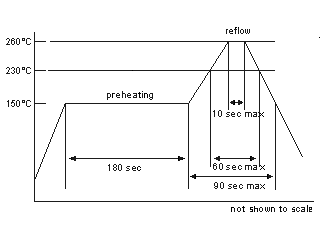
\includegraphics[width=0.5\textwidth]{reflow.png}
\caption[\url{http://www.comtec-crystals.com/images/service/reflow.gif}]{Temperaturkurve für Reflowlöten}\label{reflow}
\end{figure} \\
Da die Leiterplatte doppelseitig ist, kann man hier nicht auf beiden Seiten das Reflow-Verfahren benutzen. Deshalb wurde Zuerst auf der Rückseite Lötpaste für den microSD-Karten Slot und dem Quarzoszillator aufgetragen. Nachher wurden die Komponenten platziert. Dann wurden diese mit dem Heissluftföhn verlötet (siehe Abb.\ref{unterlot}). Um das Herausfallen der Teile im Ofen zu verhindern werden sie mit hitzebeständigen Klebeband fixiert. \\
\begin{figure}[h]
\centering
\includegraphics[width=0.5\textwidth]{unterlot.jpg}
\caption[Eigenes Bild]{Löten des Quarzes und des microSD-Karten Slots}\label{unterlot}
\end{figure} \\ \\
Dann wurde auf einer Holzplatte Löcher an den Positionen der Verlöteten Komponenten gebohrt. Damit wird erreicht, dass man die Vorderseite, Plan auf dieser Holzplatte gelegt werden kann. Mit den restlichen PCBs, man kann nur fünf auf einmal bestellen, wurde ein Rahmen erstellt, um so das teilweise gelötete Board zu fixieren. Dann wurde die Schablone ausgerichtet und festgemacht. So konnte man mit Lötpaste und einem Spachtel, die Löcher und somit auch die Lötstellen mit Lötpaste füllen (siehe Abb.\ref{schabi}). 
\begin{figure}[h]
\centering
\includegraphics[width=0.5\textwidth]{schabi.jpg}
\caption[Eigenes Bild]{Mit Hilfe des Spachtel und der Schablone aufgetragene Lötpaste.}\label{schabi}
\end{figure} \\
Dann wurde die Schablone entfernt. Mithilfe des Mikroskops wurden die Teile dann auf der Leiterplatte plaziert (siehe Abb.\ref{plati}). 
\begin{figure}[h]
\centering
\includegraphics[width=0.5\textwidth]{plati.jpg}
\caption[Eigenes Bild]{Bestückes PCB}\label{plati}
\end{figure} \\
Im Ofen wurden sie dann ungefähr nach der Temperaturkurve gebacken und so war die Vorderseite gelötet (siehe Abb. \ref{vordi}). \\
\begin{figure}[h!]
\centering
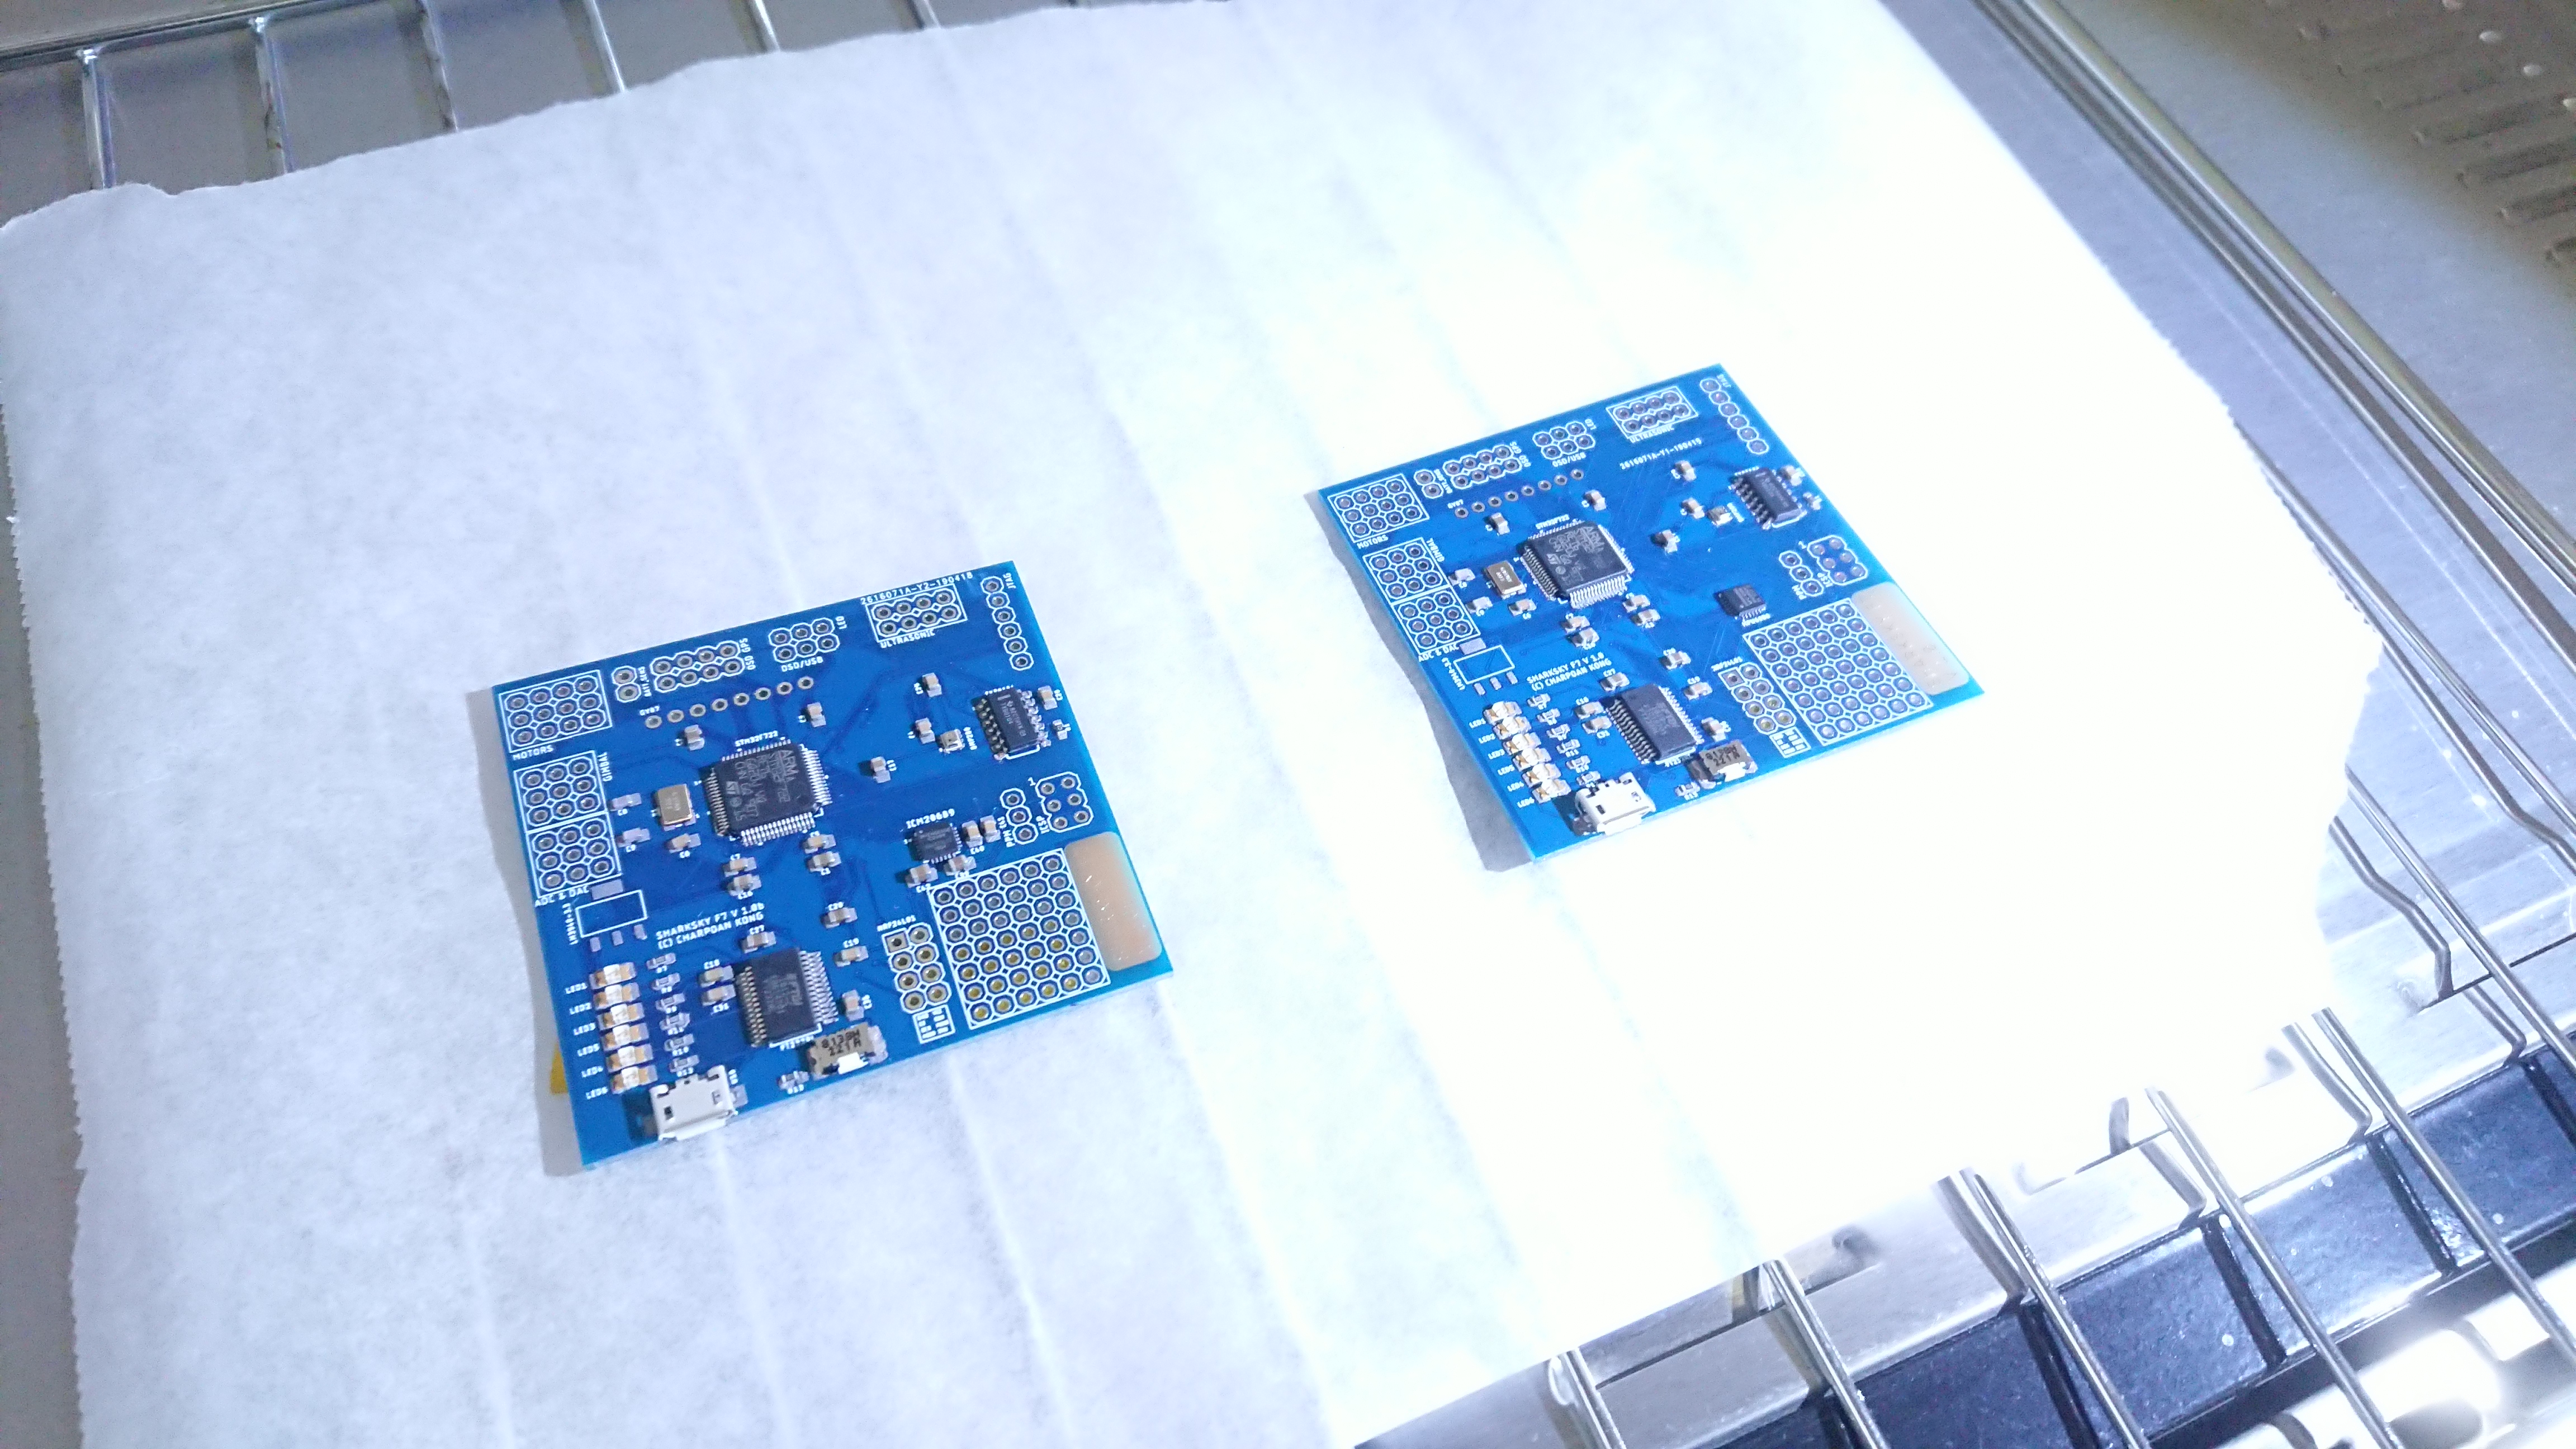
\includegraphics[width=0.5\textwidth]{vordi.jpg}
\caption[Eigenes Bild]{Gelötete Vorderseite}\label{vordi}
\end{figure} \\ 
Die Hinterseite wurde dann per Hand fertig gelötet. Dann wurden nur noch die Konnektoren angelötet und der Flightcontroller ist fertig zum programmieren (siehe Abb.\ref{fertig}).
\begin{figure}[h!]
\centering
\includegraphics[width=0.5\textwidth]{fertig.jpg}
\caption[Eigenes Bild]{Fertiges Lightcontroller Board}\label{fertig}
\end{figure} \\
\newpage
\subsubsection{Programmierung}
Der FC wird mit C und C++ programmiert. Dabei wurde die STM32CubeIDE von STMicroelectronics benutzt, die eine Eclipse IDE mit den entsprechenden Bibliotheken vorinstalliert ist. Es wurden für die einzelnen Komponenten auch andere Bibliotheken benutzt, die z.t. für den STM32 umgeschrieben werden mussten. Die Bibliothek für die IMU wurde aber selbst programmiert. Dabei kamen mehrere Probleme auf, z.B. dass das ChipSelect-Signal zu früh auf High ging. In diesem Kapitel geht es um die grössten Hürden und wichtigsten Abläufe bei der programmierung des Quadrocopters. Im Listening 1 wird der grobe Ablaufplan des Programms gezeigt.

\begin{lstlisting}[language=C++,caption=Programmablauf Pseudocode]
int main(){
	initPID_Values();
	initPeriphial();
	initIMU();
	initnRF24();
	initSD();
	
	while(true){
		loop();
	}
	return 0;
}

void loop(){
	start = elapsedticks();
	
	calcTrueangle();
	writeSD() //every 200th loopcycle; deactivated when not used
	readRadio();
	calcError();
	calcPID();
	setMotor();
	
	stop = elapsedticks();
	looptime = stop - start;
}

void setMotor(){
	if(throttle < 100){
		motspeed[0:3] = 1024;	
	}else{
		motspeed[0] = throttle + roll + pitch + yaw; 
		motspeed[1]	= throttle + roll - pitch - yaw;
		motspeed[2]	= throttle - roll - pitch + yaw;
		motspeed[3]	= throttle - roll + pitch - yaw;
	}
	
	PWM_SET(M1, motspeed[0]);
	PWM_SET(M2, motspeed[1]);
	PWM_SET(M3, motspeed[2]);
	PWM_SET(M4, motspeed[3]);
}
\end{lstlisting}
\noindent
Die IMU wird per Interrupt ausgelesen. Ein Timer gibt einen 500Hz Takt aus und nach diesem liest der Microcontroller die IMU aus.
\newpage
\paragraph{Motoren und Timing}
Die ESC's der Motoren müssen mit dem OneShot125 Protokoll\cite{website:OL_OneShot125} angesprochen werden. Bei dem wird ein PWM-Signal von 2khz erzeugt. Der Nullpunkt, bei dem die Motoren aus sind, liegt bei einer Periode von 125us bzw. einem PWM von 25$\%$ (vgl. Abb.\ref{pwm}). Die Motoren erreichen ihre maximale Drehzahl bei einer Periode von 500us bzw. bei einem PWM von 50$\%$.
\begin{figure}[h]
\centering
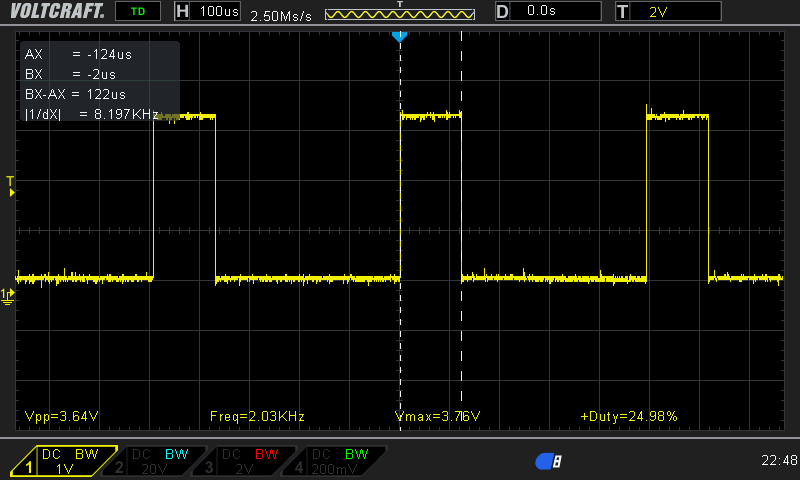
\includegraphics[width=0.9\textwidth]{PWM_25.png}
\caption[Eigenes Bild]{Signal fur die Motoren(25$\%$ PWM).}\label{pwm}
\end{figure}
\paragraph{PID Implementierung}
Der PID-Regler wird für den absoluten Winkel und für die Winkelgeschwindigkeit implementiert, wobei man die Gierachse nur mit der Winkelgeschwindikeit implementieren kann, da keine Referenz besteht, z.b durch ein Magnetometer. Die Regelungsdifferenz und Regelungskorrektur wird jeden Loop-Zyklus berechnet, der mit ca. 1.5kHz läuft.
\newpage
\subsection{Fernbedienung}
\begin{wrapfigure}[17]{r}{0.5\textwidth}
\centering
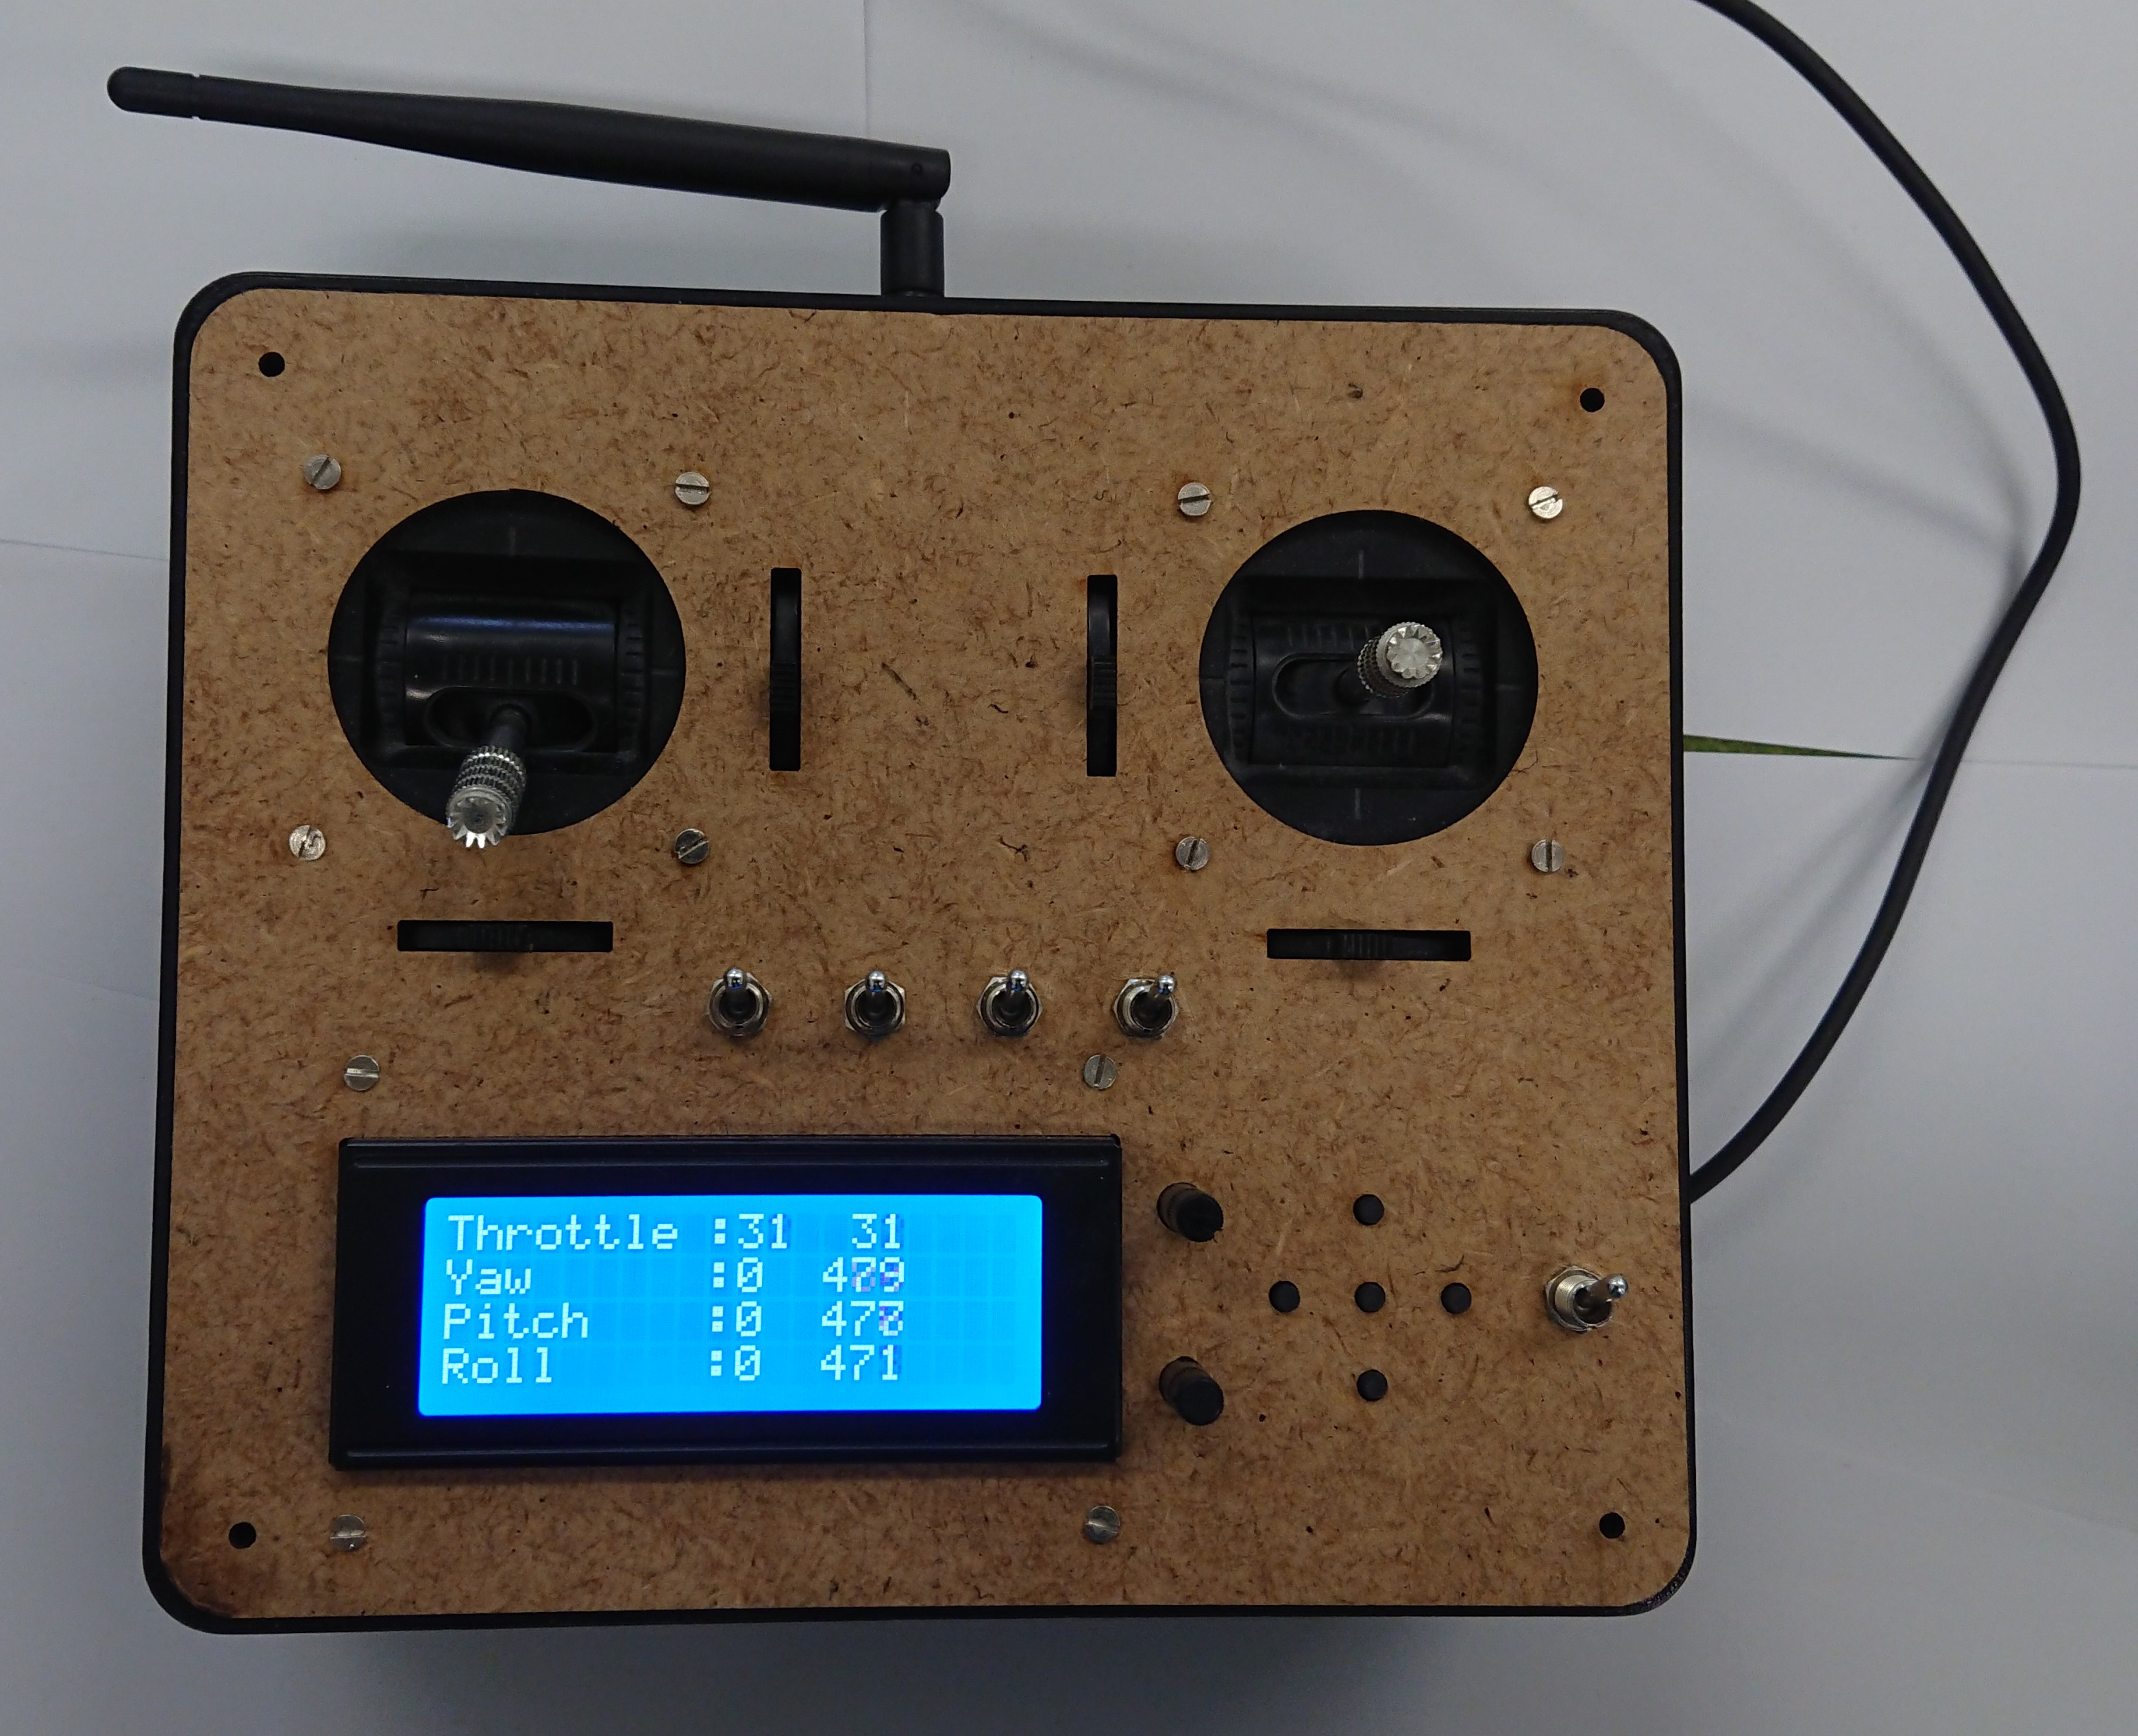
\includegraphics[width=0.5\textwidth]{Ferni.JPG}
\caption[Eigenes Bild]{Fernbedienung mit Schiebereglerausgabe auf dem Display.} \label{ferni}
\end{wrapfigure}
Die Fernbedienung (Abb.\ref{ferni}) wird aus Holz und PLA gebaut. Der Rahmen wurde mittels eines 3D-Drucker gedrukt. Das Frontpanel ist aus Holz gelasert worden. Die Schieberegler wurden aus einer kaputten Fernbedienung genommen. Auch besitzt diese ein LCD-CharDisplay mit 20x4 Zeichen. Dies wird benutzt um den genauen Ausschlag der Schieberegler, die Sensorwerte und die PID-Werte anzuzeigen bzw. zu bearbeiten. Als Microcontroller wird ein STM32F767ZI benutzt, der auf einem Nucleo-144 Protoboard verbaut ist. Listening 2 zeigt den Ablaufplan des Programmes.\\ \\ \\
\begin{lstlisting}[language=C++,caption=Programmablauf Pseudocode]
int main(){
	initPeriphial();
	initADC();
	initnRF24();

	while(true){
		loop();
	}
	
	return 0;
}

void loop(){
	readADC();
	sendData();
	
	menu_print();
}

void menu_print(){
	MENU_1:
		print_ADC_VAL();
	MENU_2:
		print_ACK_VAL();
	MENU_3:
		print_PID_ROLL_PITCH(); //<-- ALSO EDIT VALUES ON 0% Throttle
	MENU_4:
		print_PID_YAW(); //<-- ALSO EDIT VALUES ON 0% Throttle
}


\end{lstlisting}
\newpage

\subsection{Filtersimulation}
Die Filtersimulation ist ein kleines Python-Programm, das den DLPF Filter auf die aufgezeichneten Werte anwendet und ein Graph zeichnet, der die rohen Werte und die gefilterten Werte darstellt.(Bild FilterGraph). Listening 3 zeigt den Code des Programmes. 
\begin{lstlisting}[language=Python,caption=Filtersimulation]
from matplotlib import pyplot as plt
import numpy as np
import math


def digital_low_pass(cutoff_frequency, input):
    fc = 2 * math.pi * cutoff_frequency
    alpha = (fc * dt) / (1 + fc * dt)
    output = [0] * len(input)
    output[0] = input[0]

    print(alpha)

    for i in range(1, len(input)):
        output[i] = alpha * input[i] + (1 - alpha) * output[i - 1]
    return output


with open('LOG3','r') as file:
    line = []
    for i in file:
        line.append(i.rstrip('\n'))

time = []
dtime = []
dt = 0

pitch = []

for i in line:
    x = i.split('\t')
    pitch.append(float(x[0]))

for i in range(1, len(time)):
    dtime.append(time[i]-time[i-1])

for i in dtime:
    dt += i

dt = dt/len(dtime)
freq = 1.0/dt

fpitch = digital_low_pass(80, pitch)

plt.plot(time, pitch)
plt.plot(time, fpitch)

plt.show()
\end{lstlisting}
\section{Versuche}
Nach dem Bau des Quadrocopters und der Fernbedienung, wurden Tests in der Turnhalle der Schule gemacht, da der Quadrocopter schwerer als 0.5kg ist und dies gegen die Bestimmungen des Bundesamtes für Zivilluftfahrt ist, wurde desshalb auch eine Indoordrohne gebaut. \\ \\ Zuerst wurden Versuche gemacht, um den richtigen Wert des P-Reglers der Nick-und Rollachse zu bestimmen. Der Wert wurde so lange erhöht, bis der Quadrocopter zu oszillieren begann. Dann wurde er in die Mitte der Turnhalle gestellt und es wurden die ersten Flugversuche gestartet. Später wurde probiert das D-Glied einzustellen. Auch nach der Achsenkorrektur, die später in den Ergebnissen besprochen wird, waren diese Versuche gescheitert. \\ \\ In einem zweiten Versuch wurde der Quadrocopter mit einem komerziellen Quadrocopter des Mechanikers verglichen. Dadurch wurden einige Fehler, die im Kapitel 
Ergebnisse besprochen werden, korrigiert. Durch diese Korrektur kam es zu einem halberfolgreichen Versuch. \\ \\ Die Gierachse wurde auch im ersten Versuch getestet. Dabei wurde bemerkt, dass diese zu stark reagierte. Der Mechaniker hat dann behauptet, dass die Gierachse auf 5Hz gefiltert werden muss. Dabei wurde ein kleines Python-Programm geschrieben, dass die aufgezeichneten Werte filterte. Natürlich konnte so nicht der Effekt des Filtes simuliert werden. Diese Versuche waren nicht befriedigend und so wurde das Augenmerk zunächst auf die Nick-und Rollachse geworfen. \\ \\ Beim leztzen Versuch ist es leider zu einem Unfall gekommen und einer der Motoren wurde beschädigt, somit kann auch die Versuchsreihe bis zur Abgabe der Maturarbeit nicht weitergeführt werden, da die Motoren eine lange Lieferfrist haben und auch ein neuer Rahmen von Vorteil ist, da beim alten die Beine beschädigt waren und nicht richtig repariert werden konnten. Somit ist der Quadrocopter bis zur Abgabe noch nicht flugfähig. 
\newpage

\section{Ergebnisse}
Die erste Versuchsreihe war gescheitert. Dabei spielen viele Gründe eine Rolle. Erstens wurde entdeckt, dass der Intertialsensor bei einer Gierbewegung die Nick-und Rollachse nicht ineinander übersetzt werden, wie es in Kapitel über den Intertialsensor beschrieben wird. Auch wurden die rauschigen Sensorwerte, die mit der SD-Karte geloggt wurden, entdekt. So wurde ein DLPF einprogrammiert, der die Sensorwerte filtert. Auch wurde wie vorher beschrieben eine kleine Simulation geschrieben um den Filter zu testen. Dieser lieferte dann auch bessere Sensorwerte, die nicht rauschten. Auch nach diesen Verbesserungen ist es dem Quadrocopter nicht gelungen zu fliegen. \\ \\In der zweiten Versuchsreihe wurde dann entschieden den Quadrocopter mit einem anderen zu Vergleichen der fliegt. Dabei wurde bemerkt, dass die P-Werte viel zu klein waren und so wurden sie um den Faktor fünf erhöht. Dieser zu kleine Wert zeichnete sich damit aus, dass die Reaktion beim fliegenden Quadrocopter viel stärker war als bei der selbstgebauten. \\ \\ Dennoch als der Quadrocopter mehr oder weniger flog, zeigte er ein Verhalten auf, dass dieser beim Flug oszillierte und dieser immer zu einer Seite driftete. Dieses Verhalten konnte nicht mehr weiter erforscht werden, da der Quadrocopter beschädigt wurde und nicht in der Frist bis zu Abgabe repariert werden kann.
\newpage
\section{Diskussion}
Da keine weiteren Versuche gemacht werden können, kann nur spekuliert werden, wieso der Quadrocopter einen unstabilen Flug absolviert hat. Die Werte waren sicher nicht optimal und das D-Glied, dass solche Oszillationen verhindern solle, war auch nicht Ideal eingestellt worden. Auch ist es möglich, dass der Filter der angewant wurde, die Regelung verzögert und somit auch die Antwort des FC's auf die Oszillationen, da auch die IMU einen DLPF besitzt und so zwei Filter in Reihe geschaltet sind. Nach der Abgabe des Schriftlichen Teils werden weitere Versuche getätigt sobald der Quadrocopter repariert ist, um so die Ursache der Oszillationen herauszufinden und diese zu korrigieren. \\ \\ Dennoch wurden viele der Ziele erreicht. Das designen und bauen des Flightcontrollers war erfolgreich und dieser zeigte auch das richtige Reglelverhalten. Auch konnte in der testfreien Phase, der Programmloop des FC's von 200Hz auf ca. 1.5kHz erhöht werden, was zu einer schnelleren Regelung führt.  \\ \\
Im Vergleich zum Flightcontroller mit dem Raspberry Pi, konnten alle Probleme gelöst werden, die dieser Verursacht hat. Es gab beim programmieren fast keine Probleme und auch wurde gelernt wie man auf der STM32-Plattform programmiert. \\ \\ Zum Schluss möchte ich mich noch an dem Physiklabroant Bruno Turnherr bedanken, der sein Wissen über Quadrocopter, PCB-Design, Reflow-Löten gezeigt hat und für die Hilfe beim Bau des Quadrocopters. 

\newpage
\section{Quellenverzeichnis}
\subsection{Literaturverzeichnis}
\printbibliography[heading=none]
\subsection{Abbildungsverzeichnis}
\makeatletter
\@starttoc{lof}% Print List of Figures
\makeatother
\newpage
\section{Anhang 1}
Auflösung 1:
\begin{align*} 
x_{i}-y_{i}&=RC\cdot \frac{y_{i}-y_{i-1}}{\Delta t} \\ 
x_{i}-y_{i}&=\frac{RCy_{i}-RCy_{i-1}}{\Delta t}\\
x_{i}\Delta t-y_{i}\Delta&=RCy_{i}-RCy_{i-1} \\
y_{i}\Delta t+RCy_{i}&=x_{i}\Delta t+RCy_{i-1} \\
y_{i}(\Delta t+RC)&=x_{i}\Delta t+RCy_{i-1} \\
y{i}&=x_{i}\frac{\Delta t}{\Delta t+RC} + y_{i-1}\frac{RC}{\Delta t+RC}
\end{align*}
Beweis 1:
\begin{align*}
\alpha&=\frac{\Delta t}{\Delta t+RC} \\
\alpha \Delta t+RC\alpha &= \Delta t \\
RC\alpha &= \Delta t \alpha \Delta t \\
RC &= \Delta t \frac{1-\alpha}{\alpha}\\
\frac{1}{2\pi f_{c}} &= \frac{\Delta t -\alpha\Delta t}{\alpha} \\
\frac{1}{2\pi f_{c}} \alpha &= \Delta t -\alpha\Delta t \\
\frac{1}{2\pi f_{c}} \alpha + \alpha\Delta t &= \Delta t \\
\alpha &= \frac{\Delta t}{\frac{1}{2\pi f_{c}} + \Delta t} \\
\alpha &= \frac{\Delta t}{\frac{1+2\pi f_{c}\Delta t}{2\pi f_{c}}} \\
\alpha &= \frac{2\pi f_{c}\Delta t}{1+2\pi f_{c}\Delta t} 
\end{align*}

\end{document}
